\documentclass{article}
\usepackage[left=2cm, right=2cm, top=2cm, bottom=2cm]{geometry}
\usepackage{graphicx} 
\usepackage{url}
\usepackage[utf8]{inputenc}
\usepackage{parskip} 
\setlength{\parskip}{0.5 cm}
\graphicspath{{Imagenes/}}

\title{\vspace{-1.5cm} Curriculum Vitae \\ \Huge{Cristobal Cortés Gómez} \\ \large{Programador y Matemático Inventor} \\ \normalsize{Orgullosamente Tapatío} \\ 
\vspace{0.3cm}
\normalsize{
legocris@hotmail.com \ $|$ \ +52 33 1115 0013 \\
GitHub: \url{https://github.com/legocris} \ $|$ \ LinkedIn: \url{www.linkedin.com/in/cristobal-cortes-gomez}
}
\vspace{-1cm}}
\author{}
\date{}

\begin{document}

\maketitle

\section*{Perfil Profesional}
Matemático con sólida formación en álgebra abstracta y teoría de la computación, complementada con amplia experiencia como programador multiplataforma y  desarrollador de videojuegos independiente. Especializado en el ecosistema de TypeScript/JavaScript para desarrollo web, Python para métodos númericos e IA, C/C++ para herramientas de bajo nivel. Acostumbrado a gestionar flujos de trabajo complejos en entornos Linux, utilizar editores de terminal altamente personalizados (Emacs, Vim) y resolver problemas de arquitectura de software, así como proyectos de automatización e ingeniería de hardware.

\section*{Habilidades Técnicas}
\textbf{Lenguajes:} TypeScript, JavaScript, C, C++, C\#, Java, Python, Fortran, R, Pascal, Node.js, HTML, LUA, CSS, Less, GML, GLSL, HLSL, CUDA. \\
\textbf{Frameworks y Librerías:} React, Redux Toolkit, Three.js, Pixi.js, Sklearn, Pytorch. \\
\textbf{Herramientas y Motores:} GameMaker Studio, Unity 3D, Processing, Blender. \\
\textbf{Sistemas y Flujo de Trabajo:} Entornos Linux (shell scripting), Git, Emacs, Vim. \\
\textbf{Hardware y Electrónica:} Controladores (ESP8266, Arduino IOT), PLC Siemens, diseño de PCBs, diagnóstico de circuitos y retrofitting de dispositivos vintage.

\section*{Idiomas}
\textbf{Español:} Nativo \\
\textbf{Inglés:} Avanzado (Comunicación fluida y técnica con clientes internacionales).

\section*{Estudios}

\textbf{2017-2025}: Licenciatura en Matemáticas en la Universidad De Guadalajara CUCEI.

Proyecto final: Análisis de conveniencia de Redes Neuronales angostas contra profundas usando el perceptrón para problemas de clasificación\\
Link: \url{https://drive.google.com/file/d/1y_D-IL4z9spmbDCHWOvdoEBr8vfhC2Ic/view?usp=sharing}\\
Link: \url{https://github.com/legocris/Archivos-Proyecto-Analisis-de-Convergencia-RN}

\section*{Trabajos}

\textbf{2025-2026}: Programador freelancer en videojuego 2d de acción 2d para aprender a programar. Su característica principal es que puedes programar los poderes del personaje con Javascript.

Cliente: Gnarled Helix LLC \\
Links: \url{https://open-sourcerer.com/} \\
Imágenes:
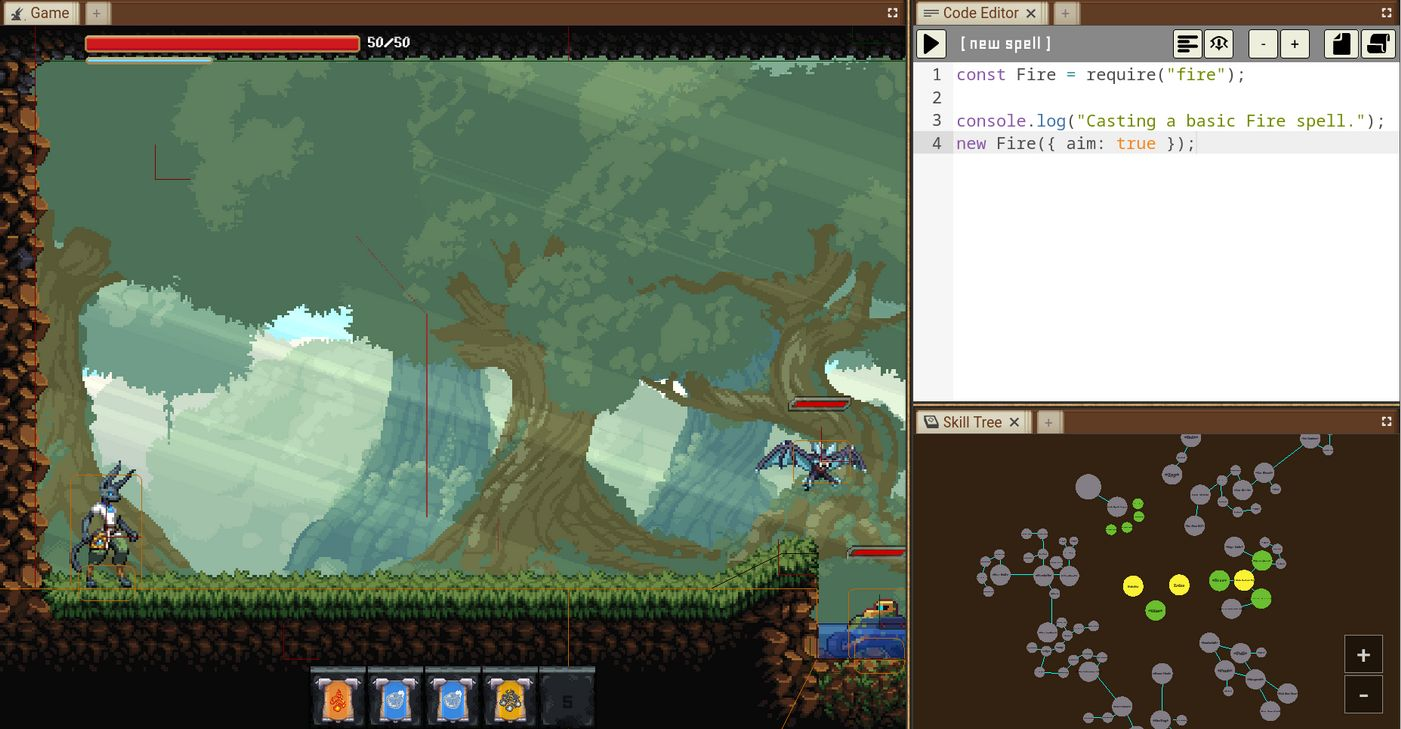
\includegraphics[width=0.45\textwidth, height=3.5cm, keepaspectratio]{Gnarled Elix.jpg}

\textbf{2024-2025}: Diseñador y único Programador de Videojuego del juego de mesa Camino a Xibalbá PITZ.

Cliente: Jalapeño Labs. \\
Links: \url{https://jalapenolab.mx/pages/pitz} \\
Tecnologías usadas: GameMaker:Studio, Javascript, Firebase. \\
Imágenes:
    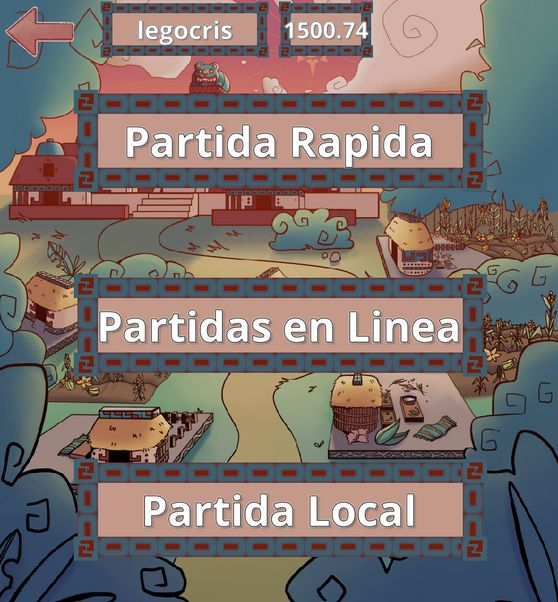
\includegraphics[width=0.35\textwidth, height=3cm, keepaspectratio]{Jalapeño0.jpg}\hspace{0.5cm}%
    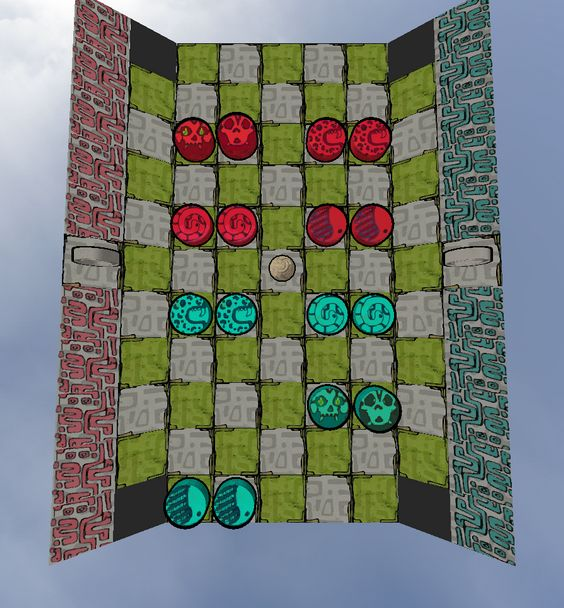
\includegraphics[width=0.35\textwidth, height=3cm, keepaspectratio]{Jalapeño.jpg}

\textbf{2023-2024}: Invernadero Automático para cultivo de hongos comestibles. Construcción de un invernadero automático con controles de humedad y temperatura para cultivar hongos con toda su instalación eléctrica.

Tecnologías usadas: Controlador esp8266, Arduino IOT, Placa PCB. \\
Video: \url{https://drive.google.com/file/d/1VXNXsHJxxcXPUsZ7u1oSj_WJdibgUq9U/view?usp=drive_link} \\
Imágenes:
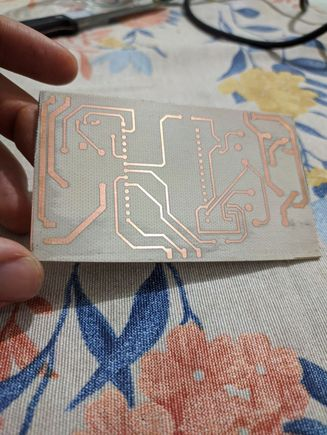
\includegraphics[width=0.25\textwidth, height=3cm, keepaspectratio]{Inti1.jpg}\hspace{0.4cm}%
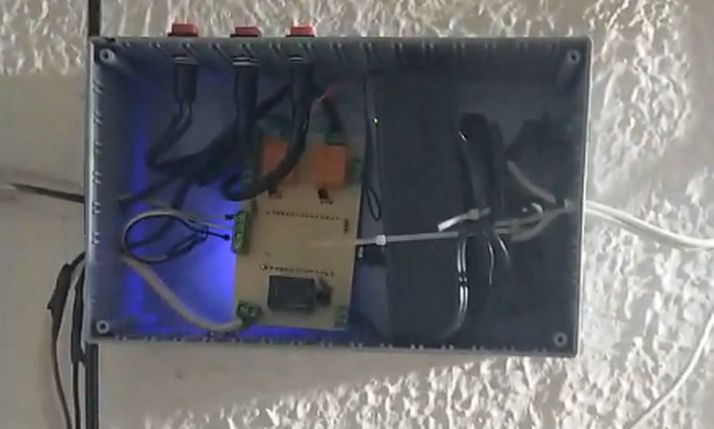
\includegraphics[width=0.25\textwidth, height=3cm, keepaspectratio]{Inti2.jpg}\hspace{0.4cm}%
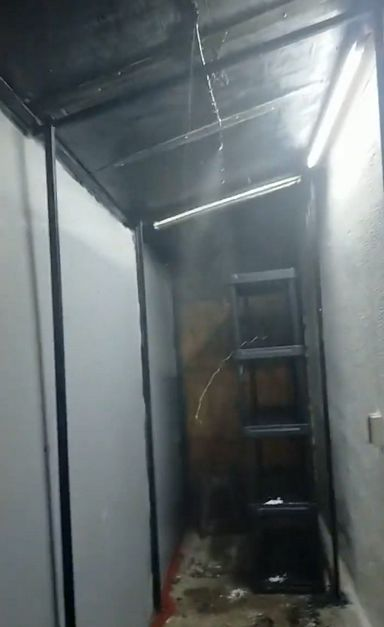
\includegraphics[width=0.25\textwidth, height=3cm, keepaspectratio]{Inti3.jpg}

\textbf{2022-2024}: Clases de matemáticas. Clases particulares de matemáticas a adolescentes y adultos.

\textbf{2022}: Clases de robótica a niños durante un semestre.

Cliente: American World Languages (Awl chapultepec) \\
Video: \url{https://drive.google.com/file/d/1jcYXvor1MOY12M_HYyBxCDk3AN8kvsEa/view?usp=sharing} \\
Imágenes:
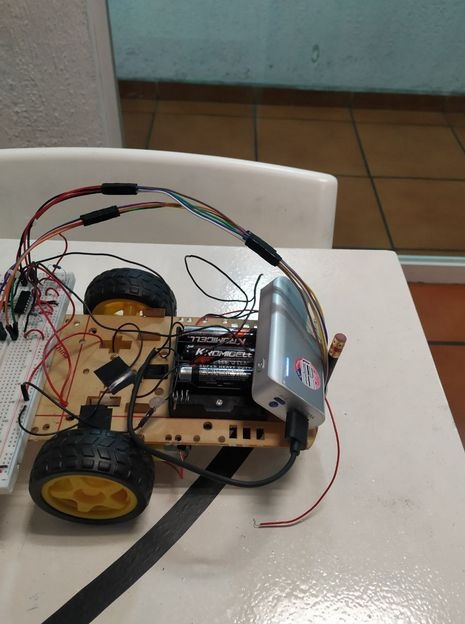
\includegraphics[width=0.45\textwidth, height=3.5cm, keepaspectratio]{AmericanWorldLanguages.jpg}

\textbf{2020-2022}: Trabajo de experimentación artística para proyecto social y artístico sobre la intersexualidad. Creación de un Cubrebocas LED en el que podrías poner simples imágenes propias. Simulador de un Museo en 3D.

Tecnologías usadas: Javascript, Arduino, controlador esp8266, Blender, Unity 3d. \\
Cliente: Proyecto INTERSEX \\
Links: \url{https://intersex.mx/}

\textbf{2017-2020}: Desarrollo de la página web para venta de Luminarias para Alumbrado Público SGT Total. Página adaptada a dispositivos móviles escrita en html+css. \\
Links: \url{https://sgt-total.com/}

\textbf{2018}: Upwork: Desarrollo completo de un pequeño videojuego que simula el escritorio de una computadora pero al dar click en un archivo el sistema se corrompe y tienes que memorizar textos que aparecen durante pocos segundos y reescribirlos.

Cliente: Daniel Douglas \\
Imágenes:
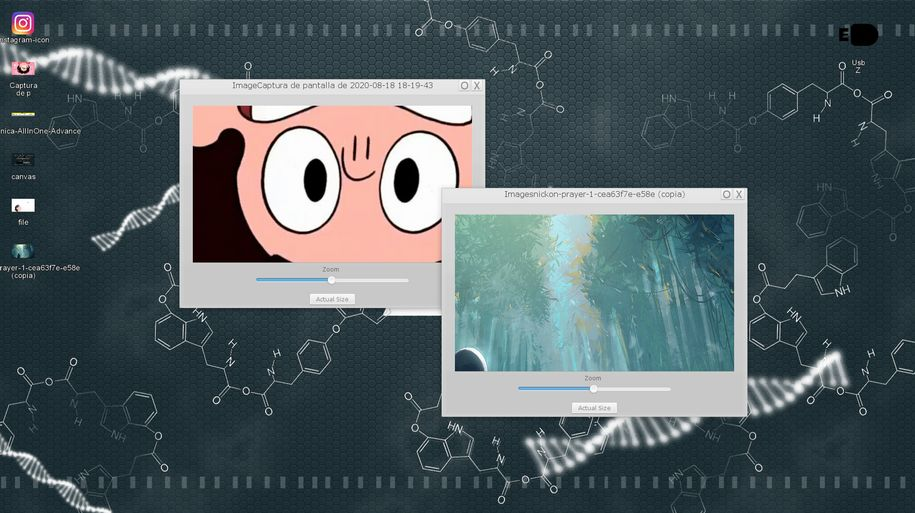
\includegraphics[width=0.35\textwidth, height=3cm, keepaspectratio]{DanielDouglas.jpg}\hspace{0.5cm}%
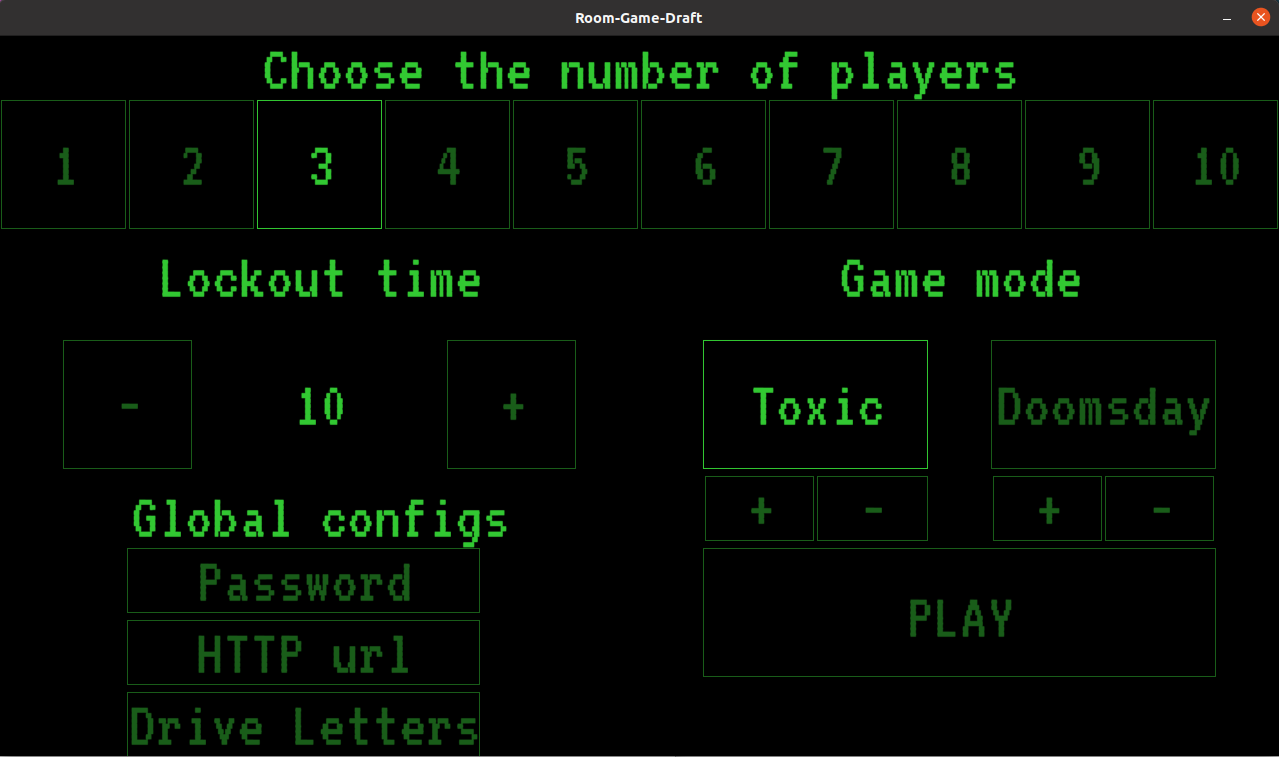
\includegraphics[width=0.35\textwidth, height=3cm, keepaspectratio]{DanielDouglas2.png}

\textbf{2017}: Función de teatro Habitar. Participación en el desarrollo de una aplicación con Kinect para hacer cambios en tiempo real a la proyección de acuerdo a los movimientos de la barra.

Cliente: Función de habitar, dirigida por Velvet Ramírez en el área de Multimedia con Selene González y Eduardo Jiménez. \\
Tecnologías usadas: Processing, Java, GLSL \\
Links: \url{https://cultura.iteso.mx/web/general/detalle?group_id=5313293}

\textbf{2018}: Upwork: Unity - Shader conversion and application. Adaptación de un script (shader) escrito en glsl al lenguaje hlsl. El propósito del script es hacer una proyección esférica o de “ojo de pescado” para usarse en lentes de realidad virtual. Es usado en una aplicación médica.

Tecnologías usadas: GLSL, HLSL, Unity3D. \\
Cliente: Immertec, Jon Clagg \\
Imágenes:
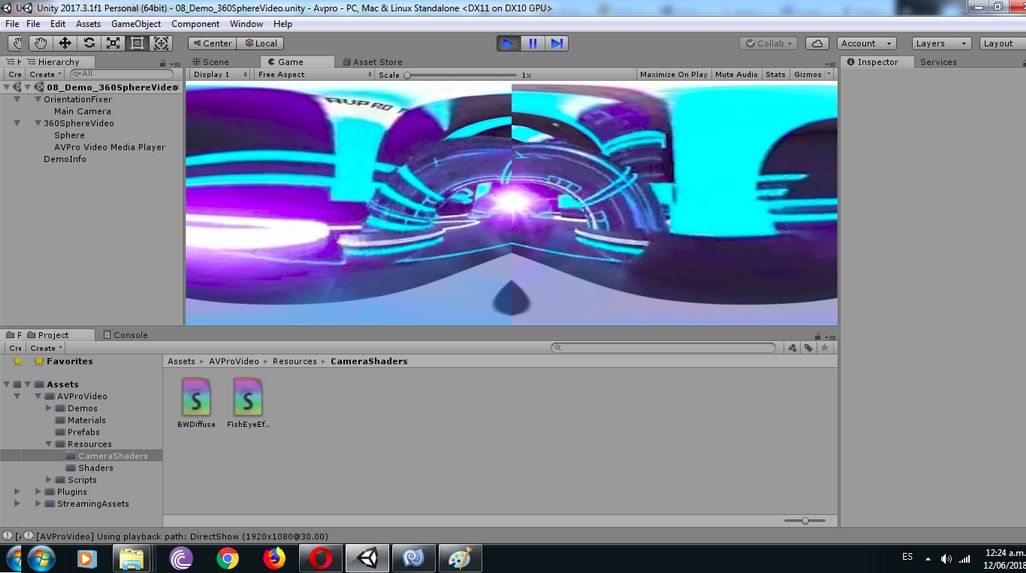
\includegraphics[width=0.45\textwidth, height=3.5cm, keepaspectratio]{Immertec.jpg}

\textbf{2016-2017}: Automatización y diseño industrial. Diseño y creación de una máquina etiquetadora de botellas semiautomática. Programación de un plc para una lava-llenadora de barriles.

Tecnologías usadas: Arduino Mega, PLC Siemens. Programación en diagrama de flujo. \\
Cliente: Cervejal \\
Video: \url{https://1drv.ms/v/s!Aslbn4nR5WV3gXMu1zZDiq8jeHbF}


\section*{Proyectos Independientes Concretados}

\textbf{2019}: Videojuego de Me Canso Ganso. Co-Programador de videojuego arcade el que manejas al Presidente López Obrador cabalgando un ganso y saltas obstáculos que se hacen cada vez más rápidos.

Tecnologías usadas: GameMaker:Studio 2, lenguaje gml. \\
Links al APK (ya no en la tienda): \\
\url{https://apkpure.com/de/me-canso-ganso/com.piratagamesparatu.mecansoganso/download/1.0.0} \\
\url{https://drive.google.com/file/d/1a3S5-g950tGvitwL9Aq6CDquU3H9GVtZ/view?usp=sharing}

\textbf{2018}: Videojuegos Sacrifice your Brothers. Co-Programador del juego arcade multijugador local de acción en el que tienes que tomar la difícil decisión de salvar a tus compañeros o sacrificarlos en una urna para adquirir más tiempo de vida.

Links: \url{https://axolotlbros.itch.io/sacrifice-your-brothers} \\
Imágenes:
\begin{center}
    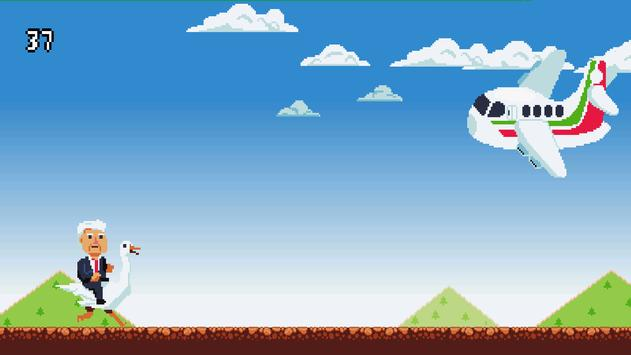
\includegraphics[width=0.25\textwidth, height=3cm, keepaspectratio]{AxolotlBros1.png}\hspace{0.4cm}%
    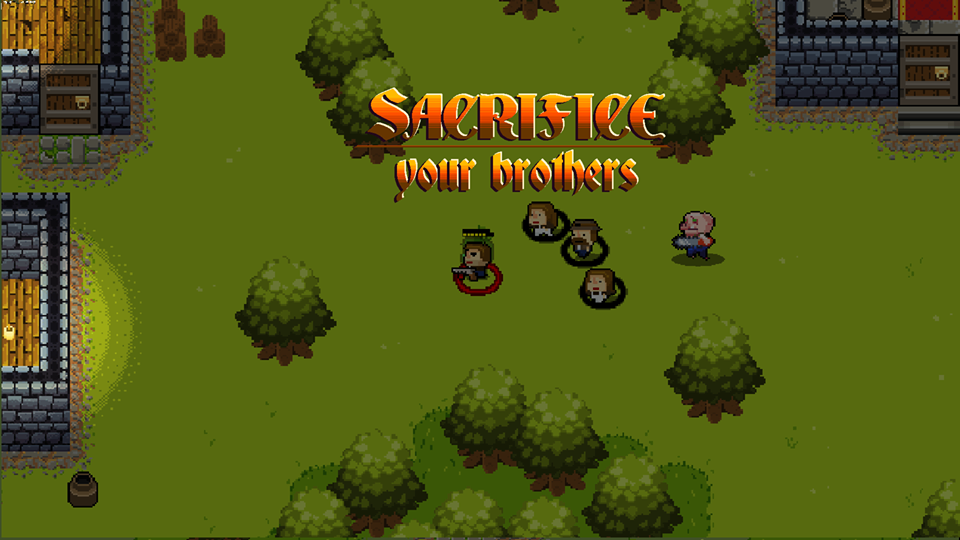
\includegraphics[width=0.25\textwidth, height=3cm, keepaspectratio]{AxolotlBros2.png}\hspace{0.4cm}%
    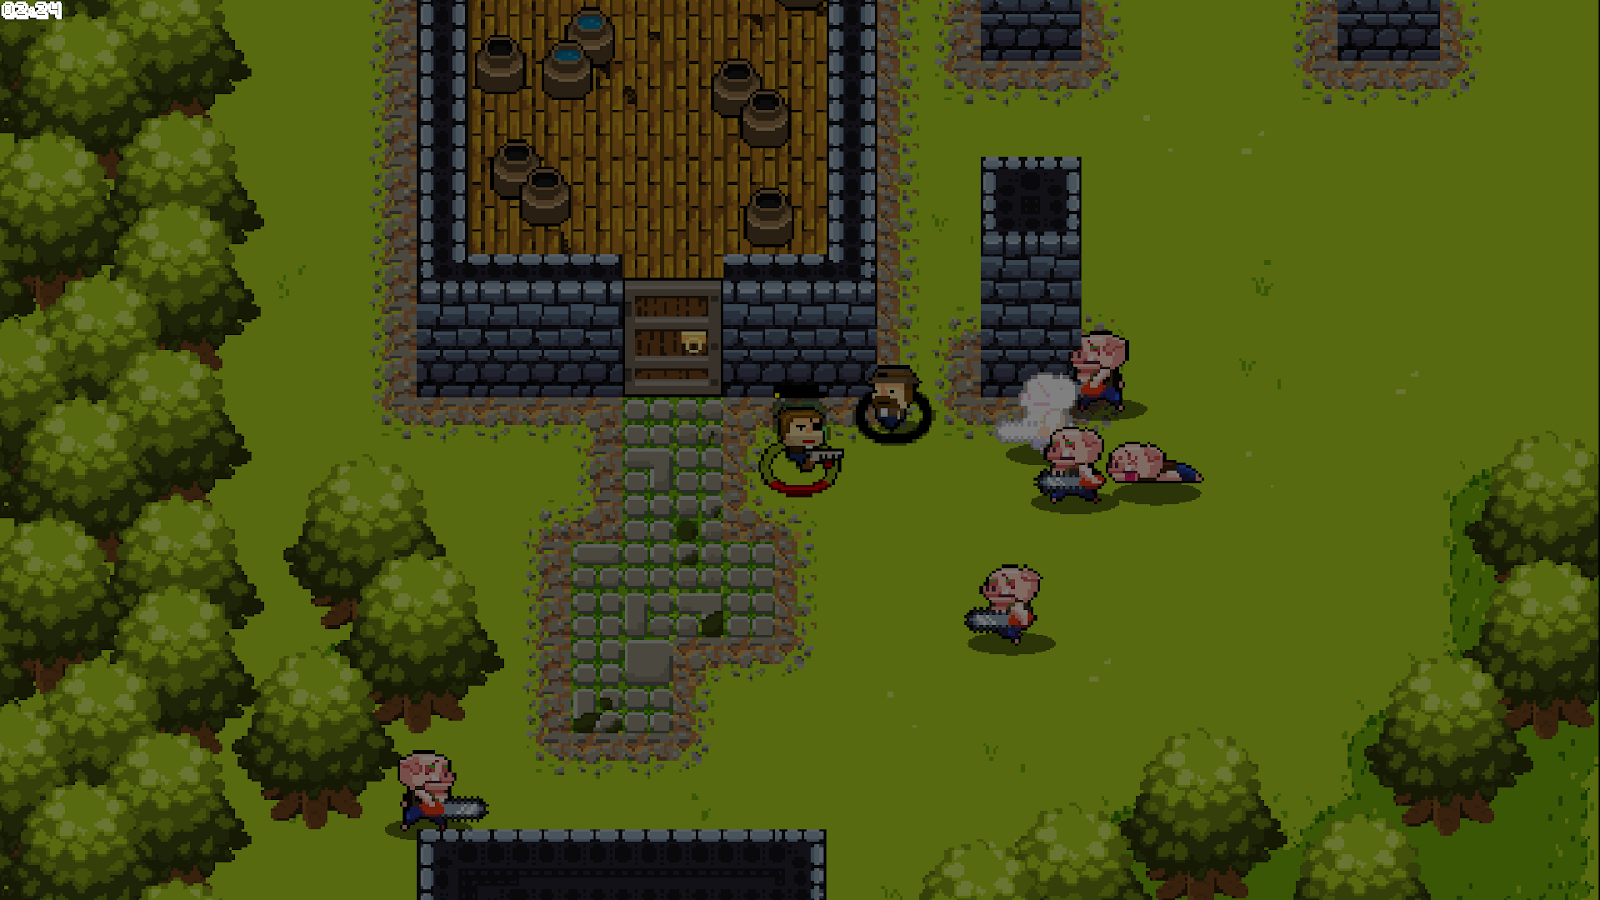
\includegraphics[width=0.25\textwidth, height=3cm, keepaspectratio]{AxolotlBros3.png}
\end{center}

\textbf{2014}: Videojuego Sweet Valentine’s Day. Toda la programación del juego arcade para móviles en el que eres cupido y debes de conectar a la mayor cantidad de parejas y evitar que otros arruinen el amor usando tu flecha que los elimina.

Links al APK (ya no en la tienda): \\
\url{https://apkpure.com/sweet-valentine-s-day-free/com.axolotl.svdayfree} \\
\url{https://drive.google.com/file/d/1MA1SfxKcKKX8VI8fpP4RzvQA85vqMPDv/view?usp=sharing}\\
Imágenes:
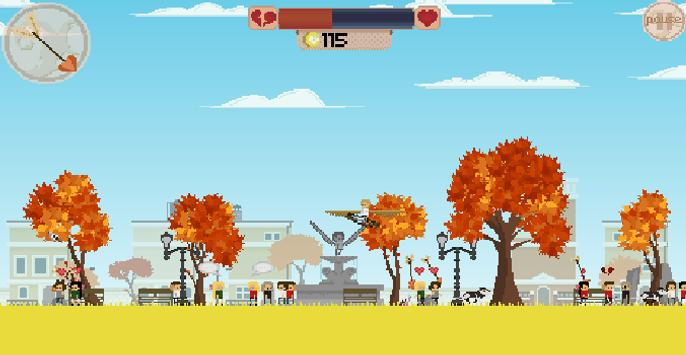
\includegraphics[width=0.35\textwidth, height=3.5cm, keepaspectratio]{AxolotlGames.png}

\textbf{2012}: Videojuego Morbus. Videojuego survival arcade en el que debes de sobrevivir a hordas de zombis equipado con armas que vas mejorando conforme obtienes dinero. Participó en el concurso Proyecto Multimedia y ganó medalla de bronce en \textbf{2012}.

Link al ejecutable: \url{https://drive.google.com/file/d/1DNkXIkSf1YP37GFBk0NhI1SNT005FhZE/view?usp=sharing} \\
Imágenes:
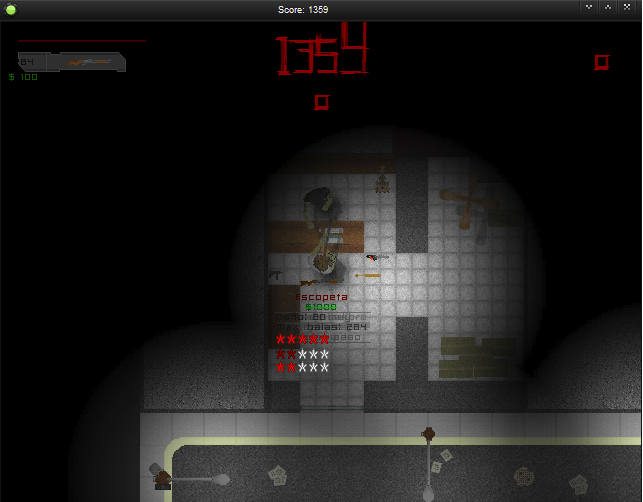
\includegraphics[width=0.45\textwidth, height=3.5cm, keepaspectratio]{ProyectoMultimedia.png}

\section*{Cursos y Actualizaciones Académicas:}
Escuela de Matemáticas de Occidente (EMO 2024) (40 hrs): \\ 
Link: \url{https://www.facebook.com/share/p/194nTvHzMR/} \\
PredGenIA (2023) Métodos de Aprendizaje Profundo para Predicción Genómica (20 hrs). \\ Link: \url{https://silo.uy/vufind/Record/REDI_9e7d18e2dc02c81f054dbc56c7acd0d1/Details?sid=7802947} \\
VI Escuela de Verano en Matemáticas CUCEI (2022 y 2023) Formación intensiva (60 hrs): \\
Link: \url{https://www.cucei.udg.mx/carreras/matematicas/es/video/escuela-de-verano-en-matematicas}

\section*{Otros Links}
Entrevista en GAME DEV XPerience \textbf{2018} UNAM: \\
\url{https://www.youtube.com/watch?v=Jzu9Uo8_aTk}

Juegos de Global Game JAMS en 48hrs (desde \textbf{2012}): \\
\url{https://www.youtube.com/watch?v=sKryIP7iI3w} \\
\url{http://2013.globalgamejam.org/2013/sweet-valentines-day} \\
\url{http://globalgamejam.org/2016/games/devils-best-friend}\\
\url{https://v3.globalgamejam.org/2018/games/chromobot-fighters-roboffice-edition}\\
\url{https://v3.globalgamejam.org/2019/games/la-casa-del-roboritmo}\\
\url{https://v3.globalgamejam.org/2020/games/pits-fire-4}\\
\url{https://globalgamejam.org/games/2024/comrade-spatial-baby-9}


Proyecto independiente AXOLOTL BROTHERS:
\url{https://www.youtube.com/@axolotlbrothers1253} \\
\url{https://axolotlbros.itch.io/} \\
\url{https://www.facebook.com/AxolotlBros/} \\
\url{https://x.com/axolotlbros?lang=ar-x-fm}

\end{document}